\begin{frame}[label=metho]{Methodology}
	\textbf{Project Pipeline}
	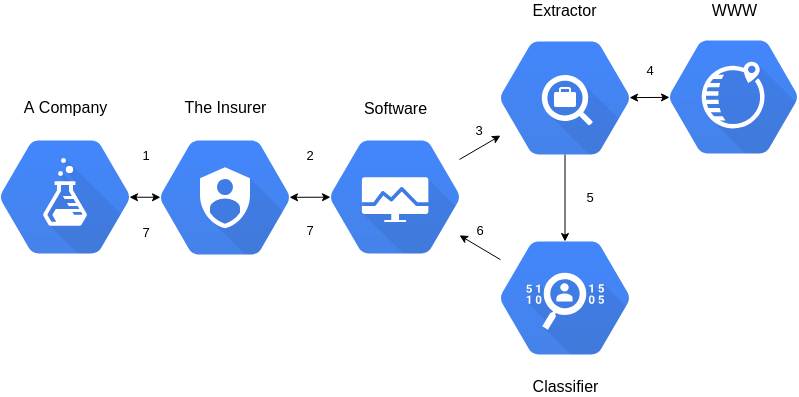
\includegraphics[width=\textwidth]{images/project_pipeline.png}
\end{frame}


\begin{frame}[label=metho]{Methodology}
	\textbf{The Extractor}
	\begin{itemize}
		\item Lot of work
		\item No Universal extractor
		\item Multistep extraction process
	\end{itemize}
\end{frame}


\begin{frame}[label=metho]{Methodology}
	\textbf{Extraction Example}
	
\end{frame}



\begin{frame}[label=metho]{Methodology}
	\textbf{Automating Extraction}
	\begin{itemize}
		\item Crawler and Scrapers
		\begin{itemize}
			\item Mimics the user by browsing without browser
			\item limitations: user interface design, dynamic rendered content and capcha
		\end{itemize}		
		\item Application Programming Interface (API)
		\begin{itemize}
			\item API based economy
			\item Communication contract
		\end{itemize}	
		\item Extraction Software should support both methods of extraction
	\end{itemize}	
	
\end{frame}



\begin{frame}[label=metho]{Methodology}
	\textbf{Using Textual Data}
	\begin{itemize}
		\item Linking key words to categories 
		\item Using the dynamic descendent classification framework
	\end{itemize}	
	
	\textbf{Dynamic descendent classifier}
	\begin{itemize}
		\item Machine Learning Algorithm trained to predict class based on words
		\item convert words into numeric vector
		\item generate a prediction based on the vector's values
	\end{itemize}	
	
\end{frame}


\begin{frame}[label=metho]{Methodology}
	\textbf{Training an algorithm}
	\begin{itemize}
		\item Classification is a task requiring supervised learning
		\item Requires a set of $N$ example with their good answer
		\item Calibrate itself to minimize loss function
	\end{itemize}	
	
	\textbf{Algorithm Trained by Supervised Learning}
	\begin{itemize}
		\item Be $\textbf{X}$ a $N\times M$ matrix, with $N$ the number of example and $M$ features
		\item Be $\textbf{Y}$ a $N\times1$ column vector, containing the associated values of the $N$ examples
		\item Let the algorithm \textit{learn} the $\beta$ that minimize the Mean Square Error in 
		$$ \textbf{Y} = \beta\textbf{X} $$
		\item Arguably, the $\beta$ are obtained with the Maximum Likely Hood estimators
	\end{itemize}	
	
\end{frame}


\begin{frame}[label=metho]{Methodology}
	\textbf{Building a Training Data Set}
	\begin{itemize}
		\item Need to create a dataset 
		\begin{itemize}
			\item Linking a company occupation, as defined by a classification scheme
			\item To keywords extracted from a source
		\end{itemize}	
		\item The Dataset is source specific
		\item Small to Medium Data
	
	\end{itemize}	
\end{frame}


\begin{frame}[label=metho]{Methodology}
	
	\textbf{Not Using Big Data in Machine Learning}
	\begin{itemize}
		\item Unrelated, yet linked concept
		\item Machine Learning is the concept of training algoritmm for specific task
		\item Big Data refers to Data with usage problem due to the 4Vs
		\begin{itemize}
			\item However, value locked in big data can be accessed using Machine Learning
		\end{itemize}	
	\end{itemize}
	
	
\end{frame}






